\chapter{Aspectos Históricos da Improvisação de códigos}\label{sec:protohistoria}

Este capítulo será dedicado à construção de um espaço conceitual histórico, do ponto de vista musical. Isto é, aqueles exemplos citados como ``proto-históricos'' que possuem alguma similaridade com o conjunto de regras práticas publicadas por \citeauthoronline{ward_live_2004} \ver{sec:laptoptoplap}. \citeonline{mori_pietro_2015} descreve um caso prematuro de \emph{live coding} na Itália, com o compositor Pietro Grossi \ver{sec:grossi}. Grossi sacrificou a questão timbrística para trabalhar na questão performática. As atividades de grupos como \emph{The Hub} \ver{sec:baiasaofranscisco}, e o compositor Ron Kuivila \ver{sec:kuivila}, no final da década de setenta e início dos anos oitenta, são descritas como fundamentais para um a construção do espírito de uma época, onde o computador se torna parte da performance musical.


\section{Pietro Grossi}\label{sec:grossi}

Pouco conhecido no contexto geral da música européia, o compositor Pietro Grossi foi  um dos pioneiros da \emph{Computer Music} Italiana. O pensamento musical que rege seus programas de computador sacrifica questões timbrísticas para concentrar na performance. Nas palavras de \citeonline[p.~126]{mori_pietro_2015}:

\begin{citacao}
\traducao{Grossi começou a se interessar por música computacional durante a primeira metade doas anos 60, quando ele quando ele organizou um programa de rádio centrado em torno da "música inovadora" em geral \cite{giomi_conversasioni_1999}. Contudo a primeira experiência de Grossi com um computador foi em Milão, no Centro de Pesquisa Elétrica da Olivetti-General. Aqui, auxiliado por alguns técnicos internos e engenheiros, ele conseguiu compor e gravar alguns de seus primeiros trabalhos em música computacional. Eles foram, em sua maior parte, transcrições de música clássica ocidental. Contudo, houve algumas exceções, por exemplo, uma faixa chamada Mixed Paganini}{Grossi began to be interested in computer music during the first half of the 1960s, when he hosted a radio program centred around “innovative music” in general (Giomi1999). However, the first Grossi's experience with calculator took place in Milan, in the Olivetti-General Electric Research centre. Here, aided by some internal technicians and engineers, he managed to compose and record some of his first computer music works. They were, for the most part, transcriptions of Western classical music. However, there were some exceptions, for example a track called Mixed Paganini.}
\end{citacao}

Existe um exemplo na \emph{internet}\disponivelem{https://www.youtube.com/watch?v=ZQSP_wF7wSY}. Um disco realizado no Studio di Fonologia musicale di Firenze, entitulado ``GE-115 - Computer Concerto'', lançado pela Olivetti em 1967: \traducao{Do lado A existem algumas transcrições de música clássica, e do lado B existem três canções originais. (\ldots) Este 7'' foi distribuído como presente de natal e de ano novo pela companhia Olivetti.}{On side A there's transcribed classical music, on side B there are three original songs. (\ldots). This 7" was distributed as a christmas and new year gift by the Olivetti company.}. No entanto, é necessária uma correção sobre o lado A, e um detalhe do lado B\disponivelem{https://www.discogs.com/Studio-Di-Fonologia-Musicale-Di-Firenze-GE-115-Computer-Concerto/release/575632}. As transcrições realizadas foram da \emph{Oferenda Musical BWV 1079} de J.S.Bach e um dos 24 Capriccio de Nicolò Paganini : \emph{i})Canon a 2 \emph{Super Thema Regium}; \emph{ii})Canon Perpetuum a 2 \emph{Quaerando Invenietis}; \emph{iii}) Canon a 3 \emph{Super Thema Regium} e; \emph{iv}) Capriccio n$^o$ 5. Das peças compostas:  \emph{i})\emph{Mixed Paganini}; \emph{ii}) \emph{Permutations Of Five Sounds} e; \emph{iii}) \emph{Continuous}.


Mori explica que a peça \emph{Mixed Paganini} derivou da transcrição do quinto \emph{capriccio}: \traducao{Praticamente, Grossi modificou, auxiliado por alguns programas rudimentares, o material sonoro original. (\ldots) Uma coleção posterior dos Capricci de Paganini, gravado em Pisa, foi revista por Barry Truax na Computer Music Journal \cite{truax_barry_1984}}{Practically, Grossi modified, aided by some rudimental music programs, the original sound material. (\ldots) A later collection of Paganini’s Capricci, recorded in Pisa, was reviewed by Barry Truax on Computer Music Journal (Truax1984).} O tipo de material sonoro utilizado nestas peças possue uma metodolgia tradicional, se comparado com os trabalhos de compositores e pesquisadores como Lejarn Hiller, Max Mathews e Michael Koenig. Por exemplo, as pesquisas desenvolvidas por \cite{mathews_digital_1963}\footnote{\cfcite{mathews_technology_1969,roads_interview_1980,park_interview_2009,di_nunzio_genesi_2010}} se preocupavam com a questão timbrística. Grossi diverge: recorre às técnicas canônicas do Período Comum (séc. XVII-XX, \emph{circa}), isto é, inversão, retrogradação, retrogradação da inversão, aceleração, diminuição, com um só timbre. 

Grossi desenvolveu o DCMP (\emph{Digital Computer Music Program}) e, segundo Mori (\emph{idem}, \emph{ibdem}), ao usar este programa, o compositor escolheu deliberadamente abandonar o problema do timbre. Esta abordagem parte de uma abordagem ``preguiçosa'' (\emph{prigo}). Grossi dizia sobre si mesmo, como ``uma pessoa que está consciente de que o seu tempo é limitado e não quer perder tempo em fazer coisas inúteis ou na espera de alguma coisa quando não é necessário.''\footnote{Tradução nossa de \emph{a person who is aware that his or her time is limited and do not want to waste time in doing useless things or in waiting for something when it is not necessary.}}. Neste sentido, defendia que o desenvolvimento de novos timbres gerados por computador deveria esperar por melhores implementações de \emph{hardware}:

\begin{citacao}
\traducao{(\ldots) o intéprete era capaz de produzir e reproduzir música em tempo real, digitando alguns comandos específicos e os parâmetros composicionais desejados. O som resultante vinha imediatamente depois da operação de decisão, sem qualquer atraso causado por cálculos. Haviam muitas escolhas de reprodução no programa: era possível salvar na memória do computador peças de músicas pré-existentes, para elaborar qualquer material sonoro no disco rígido, para administrar arquivos musicais e iniciar um processo de composição automático, baseado em algoritmos que trabalham com procedimentos ``pseudo-casuais''. Existia também uma abundância de escolhas para mudanças na estrutura da peça. Um dos mais importantes aspectos do trabalho de Grossi foi que todas intervenções eram instantâneas: o operador não tinha que esperar pelo computador terminar todas operações requisitadas, e depois ouvir os resultados. Cálculos de dados e reprodução sonoras eram simultâneos. \textbf{Esta simultaneidade não era comum no campo da \emph{Computer Music} daquele tempo, e Grossi deliberadamente escolheu trabalhar desta forma, perdendo muito no lado da qualidade sonora. Seu desejo era poder escutar os sons resultantes imediatamente}.}{(\ldots) the performer was able to produce and reproduce music in real time by typing some specific commands and the desired composition's parameters. The sound result came out immediately after the operator's decision, without any delay caused by calculations. There were many reproduction choices inscribed in this software: it was possible to save on the computer memory pieces of pre-existing music, to elaborate any sound material in the hard disk, to manage the music archive and to start an automated music composition process based on algorithms that worked with “pseudo-casual” procedures. There were also plenty of choices for piece structure modifications. One of the most important aspects of Grossi’s work was that all the interventions were instantaneous: the operator had not to wait for the computer to finish all the requested operations and then hear the results. Data calculation and sound reproduction were simultaneous. This simultaneity was not common in the computer music field of that time and Grossi deliberately chose to work in this way, losing much on the sound quality’s side. His will was to listen to the sound result immediately.}
\end{citacao}

Esta abordagem será revista como uma outra sugestão, através do nome \emph{lazy evaluation} \ver{sec:jit }. No momento, substituímos o termo ``preguiçoso'' por  \emph{reflexividade}, ou a \traducao{habilidade de um programa manipular como dados algo que representa o estado do programa durante sua própria execução, o mecanismo para codificação de estados de execução é chamado \emph{reificação}.\cite[p.~1]{malefant_reflection_1996}}{the ability of a program to manipulate as data something representing the state of the program during its own execution, the mechanism for encoding execution states as data being called reification.}. Para Grossi, existe um anseio em recuperar a reflexividade entre o dedo que toca a tecla e o som resultante. 
\todo[color=red]{\tiny Situar TAU2-TAUMUS}

Por outro lado, Grossi foi além deste problema reflexivo. É importante lembrar que Grossi contribuiu para o desenvolvimento de tecnologias telemáticas \ver{sec:telepresenca}. Mori descreve uma transmissão por telefone, subsidiada por uma companhia italiana,  entre duas cidades, durante uma conferência de tecnoclogia. Esta transmissão utilizou o \emph{software TELETAU}. O \emph{software} era executado em um \traducao{um computador conectado à rede de computadores BITNET, para explorar remotamente os recursos de cálculo do computador CNR e imediatamente escutar os resultados sonoros produzidos pelo TAU2.}{a computer connected to the BITNET computer network, to exploit remotely the CNR computer calculation resources and to immediately listen the sound results produced by TAU2.}

\begin{citacao}
\traducao{$[$Pietro$]$ Grossi fez sua primeira experiência do tipo durante uma conferência de tecnologia em Rimini em 1970, onde o músico reproduzia algumas de suas composições, bem como sons randômicos, empregando um terminal de vídeo conectado pelo telefone para o computador da CNR em Pisa. A RAI, empresa de radiodifusão italiana, emprestou suas pontes de rádio $[$Comunicação entre duas antenas$]$ para enviar sinais sonoros entre Pisa e Rimini. É como se fosse o primeiro experimento de telemática musical no mundo.\cite[p.~129]{mori_pietro_2015}}{Grossi made his first experience of this kind during a conference on technology in Rimini in 1970, where the musician reproduced many of his compositions and random sounds as well, by employing a video terminal connected via telephone to the CNR's computer in Pisa. RAI, the Italian public broadcasting company, lent its powerful FM radio bridges to send back sound signals from Pisa to Rimini. It is likely to be the first official experiment of musical telematics in the world.
}
\end{citacao}



\section{Baía de São Franscisco}\label{sec:baiasaofranscisco}

A prática musical com o computador, realizada na Costa Oeste dos EUA durante os anos 1970 e 1980,  é bastante diversa daquela realizada em grandes centros europeus (como por exemplo Ircam ou o Conservatório de Haia). \citeauthoronline{brown_indigenous_2013} comentam que esta prática decorre de alguns fatores sociais. O primeiro fator seria uma diversidade musical existente na Costa Oeste dos EUA. O segundo fator é a transmissão de conhecimentos musicais propostos por Terry Riley, Pauline Oliveros e LaMonte Young, David Tudor e Gordon Mumma. Em especial, estes dois compositores propunham a utilização de  circuitos eletrônicos eles mesmos como atores musicais \cite[3$^o$ parágrafo]{brown_indigenous_2013}. Neste sentido, uma música computacional, colaborativa e livre de restrições de regras emerge em torno do \emph{Mills College} em Oakland. 

\traduzcitacao{Com o florescimento da indústria de computadores pessoais na Baía de São Franscisco, o acesso às novas tecnologias e pessoas que desenvolveram elas era talvez o melhor no mundo. Mas se para todos os jovens com fortunas como panos para suas mentes (e seus futuros) que perseguiam um excitamento aditivo na construção de máquinas eletrônicas, também existiam políticos utópicos que sonhavam com uma nova sociedade construída no livre e aberto acesso à informação, e na abrangente tecnologia baseada em sistemas inteligentes. Esta também é a cultura que deu ao mundo a música ``New Age'', uma versão aguada e comercializada das músicas com base em modos e drones que Terry Riley, Pauline Oliveros, e LaMonte Young inventaram durante os anos cinquenta e sessenta. Mas a música feita na Costa Oeste também incluiam improvisações barulhentas e livre de restrições, que sobraram das revoluções contra-culturais dos anos 60}{With the flowering personal computer industry in the Bay Area, access to the new digital technologies and to the people who developed them was perhaps the best in the world. But for all the young men with fortunes in the back of their minds (and in their futures) who pursued the addictive excitement of building electronic machines, there were also the political utopians whose dream was of a new society built on the free and open access to information, and on a comprehensively designed technology based on embedded intelligence. This was also the culture that gave the world "New Age" music, a watered-down and commercialized version of the musics based on modes and drones that Terry Riley, Pauline Oliveros, and LaMonte Young invented here during the late fifties and early sixties. But West Coast music-making also included a free-wheeling, noisy, improvisational edge left over from the counter-cultural revolutions of the sixties.}{1$^o$ parágrafo}{brown_indigenous_2013}



\subsection{The League of Automatic Composers}

Na segunda metade da década de setenta, Jim Horton começou a adquirir micro-controladores KIM-1\footnote{\emph{Keyboard Input Monitor}. Disponível em \url{http://www.6502.org/trainers/buildkim/kim.htm}.} com interesses musicais. Segundo \citeauthoronline{brown_indigenous_2013}, não demorou para que outros compositores interessado comprassem. Discussões informais posteriores, que incluiam, além de Horton, David Behrman e John Bischoff, Rich Gold, Cathy Morton, Paul Robinson, e Paul Kalbach. Em 1977 e 1978  Horton colaborou com duas peças, apresentadas no \emph{Mills College}, que interligavam sistemas musicais elaborados com os microcontroladores \ver{sec:siskim1}. A primeira peça era construída sobre algoritmos inspirados nas teorias matemáticas de Leonard Euler (séc. XVIII). A segunda peça também explorava a comunicação entre os microcontroladores, de forma que \traducao{notas ocasionais da minha $[$Bischof$]$ máquina faziam a máquina de Jim transpor atividades melódicas de acordo com minha nota base\cite[5$^o$ parágrafo]{brown_indigenous_2013}}{the occasional tones of my $[$Bischof$]$ machine caused Jim’s machine to transpose its melodic activity according to my "key" note.}. Em 1978, Bischof, Gold e Horton formaram uma banda nas proximidades de Berkley. Posteriormente Behrman se junta ao trio. No dia 26 de Novembro gravam um \emph{Extended Play} (EP)\footnote{Gravação muito longa para um \emph{demo} e insuficiente para um disco de vinil da época.} de quatro faixas no \emph{Blind Lemmon}, um ponto de encontro musical fundado em 1958\disponivelem{http://www.chickenonaunicycle.com/Berkeley\%20Art.htm}. O disco foi lançado pela pela Lovely Music (NY) em 1980 como \emph{The Hub: Computer Network Music}.  Durante este tempo, foi formado o grupo \emph{``The League of Automatic Music Composers''}\footnote{Segundo \citeonline[6$^o$parágrafo]{brown_indigenous_2013}, o nome é uma referência ao grupo ``The League of Composers'' formado por Aaron Copland nos anos 20.}, que além de  Bischof, Behrman, contava com Tim Perkis, Scot Gresham-Lancaster, Mark Trayle e Phil Stone. Mas nosso foco será a formação no trio formado por Horton, Bischof e Perkis.

\begin{figure}[!h]
  \centering
  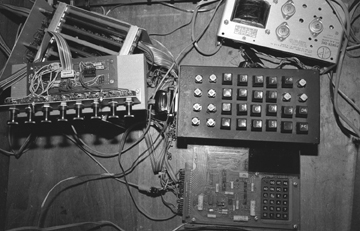
\includegraphics[scale=0.7]{imagens/siskim1.jpg}
  \caption{Sistema de música computacional de John Bischof \emph{circa} 1980. Foto: Eva Shoshanny\protect\footnotemark. \textbf{Fonte}: \citeonline{brown_indigenous_2013}.}
  \label{fig:siskim1}
\end{figure}

\footnotetext{Tradução de \emph{John Bischoff's KIM-1 computer music system circa 1980 photo: Eva Shoshany}}

É interessante uma descrição de uma performance durante 1979. Propomos aqui realizar um paralelo com \emph{happenings} (acontecimentos), manifestações artísticas já consolidadas para a época:

\begin{citacao}
Na primavera de 1979, montamos uma série quinzenal regular de apresentações informais sob os auspícios da \emph{Bay Center for the Performing Arts}. Todos outros domingos à tarde passávamos algumas horas configurando nossa rede de KIMs na sala \emph{Finnish Hall}, na Berkeley, e deixávamos a rede tocando, com retoques aqui e ali, por uma ou duas horas. Os membros da audiência poderiam ir e vir como quisessem, fazer perguntas, ou simplesmente sentar e ouvir. Este foi um evento comunitário de tipos como outros compositores aparecendo, tocando ou compartilhando circuitos eletrônicos que tinham projetado e construído. Um interesse na construção de instrumentos eletrônicos de todos os tipos parecia estar "no ar". Os eventos da sala \emph{Finn Hall} foram feitos para uma cena com paisagens sonoras geradas por computador misturado com os sons de grupos de dança folclórica ensaiando no andar de cima e as reuniões ocasionais do Partido Comunista na sala de trás do edifício velho venerável. A série durou cerca de 5 meses que eu me lembre.\cite[online]{brown_indigenous_2013}\footnote{Tradução nossa de: \emph{In the spring of 1979, we set up a regular biweekly series of informal presentations under the auspices of the East Bay Center for the Performing Arts. Every other Sunday afternoon we spent a few hours setting up our network of KIMs at the Finnish Hall in Berkeley and let the network play, with tinkering here and there, for an hour or two. Audience members could come and go as they wished, ask questions, or just sit and listen. This was a community event of sorts as other composers would show up and play or share electronic circuits they had designed and built. An interest in electronic instrument building of all kinds seemed to be "in the air." The Finn Hall events made for quite a scene as computer-generated sonic landscapes mixed with the sounds of folk dancing troupes rehearsing upstairs and the occasional Communist Party meeting in the back room of the venerable old building. The series lasted about 5 months as I remember.}}
\end{citacao}

Em 1980, Gold e Behrman abandonam o grupo, sendo que Tim Perkis se junta. Este foi período em que o grupo solidifica suas atividades na região da Baía de São Franscisco. É interessante notar que uma metodologia modular começa a ser formalizada para permitir maior flexibilidade entre os sistemas de Horton, Bischof e Perkis. Isto é, ao invés de soldar componentes eletrônicos aos controladores, os membros conectavam os microcontroladores através de portas -- o que para a época era arriscado ao ponto de queimar componentes. Com as conexões feitas, tocavam até três horas, tempo em que ouviam e ajustavam (\emph{tuning}) os sistemas em interação\disponivelem{https://www.youtube.com/watch?v=HW0qax8M68A}\cite[7$^o$ parágrafo]{brown_indigenous_2013}. Outra evento de importância é a associação do grupo com a banda \emph{Rotary Club}, formada por alunos recém-formados da \emph{Mills College}: Sam Ashley, Kenneth Atchley, Ben Azarm, Barbara Golden, Jay Cloidt e Brian Reinbolt. O grupo \traducao{baseava seu estilo de performace em torno de uma caixa de comutação projetada por Brian Reinbolt}{based their performance style around an automatic switching box designed by member Brian Reinbolt.}\cite[8$^o$ parágrafo]{brown_indigenous_2013}. Em 1983 o grupo reduziu suas atividades, época em que Horton contraiu artrite degenerativa.

\begin{figure}[!h]
    \centering
    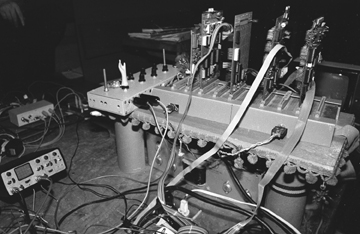
\includegraphics[scale=0.7]{imagens/perkis.jpg}
    \caption{Circuito do computador caseiro dedicado à síntese sonora de Tim Perkis, usado no começo dos anos 1980. Foto: Eva Shoshany\protect\footnotemark. \textbf{Fonte}: \citeonline{brown_indigenous_2013}}
    \label{fig:perkis}
  \end{figure}

\footnotetext{Tradução de \emph{Tim Perkis' homebuilt computer-driven sound synthesis circuitry used in early 1980s. photo: Eva Shoshany}.}

Seria possível discutir a elaboração de uma ``rede de composições''. No entanto, \citeonline[11$^o$ parágrafo] comentam que estas não eram composições específicas, mas sim concertos inteiros: \traducao{ocasiões públicas para escuta compartilhada}{public occasions for shared listening.}. Este conceito pode ser melhor compreendido através de uma descrição do processo criativo da banda, que lidavam com um sistema limitado, de \traducao{baixa velocidade 1 Mhz e poucos dados (8 bits)}{slow speed (1 Mhz) and data width (8 bits)} com uma ênfase do grupo em explorar uma luteria composicional \footnote{\cfcite{iazzetta_musica_2009,soares_luteria_2015}.} acompanhada de performance ao vivo; ou \traducao{A ênfase estava na exploração da tecnologia em mãos que poderia ser adiquirida pessoalmente ou construída a partir do zero, em vez do desejo incessante de melhores ferramentas.}{The emphasis was on exploration of the technology at hand—technology that could be personally acquired or built from scratch—rather than the endless wish for better tools.}\cite[22$^o$ parágrafo]{brown_indigenous_2013}: 

\begin{citacao}
\traducao{Os membros da liga geralmente adaptavam composições solo para usar dentro da banda. Estes solos eram desenvolvidos independentemente por cada compositor, e eram tipicamente baseados em esquemas de algoritmos de um tipo ou outro. Existiam características de improvisação diferentes para muitas delas, como bem as músicas eram diferentes em detalhes. Teorias matemáticas, sistemas de afinação experimentais, algoritmos de inteligência artificial, projetos de instrumentos de improvisação, e performance interativa eram algumas das áreas exploradas nestes trabalhos (\ldots) Os solos tocavam simultaneamente no cenário de grupo, se tornando ``sub''-composições que interagem, cada uma enviando e recebendo dados pertinentes para o funcionamento musical. \cite[12$^o$ parágrafo]{brown_indigenous_2013}.}
{League members generally adapted solo compositions for use within the band. These solos were developed independently by each composer and were typically based on algorithmic schemes of one kind or another. There was a distinctly improvisational character to many of these as the music was always different in its detail. Mathematical theories of melody, experimental tuning systems, artificial intelligence algorithms, improvisational instrument design, and interactive performance were a few of the areas explored in these solo works. (\ldots) The solos, played simultaneously in the group setting, became interacting "sub"-compositions, each sending and receiving data pertinent to its musical functioning.}
\end{citacao}

\subsection{The Hub}

\todo{\tiny Terminar a parte do the hub}

\subsection{Ron Kuivila}\label{sec:kuivila}

\citeonline{mclean_patterns_2009} comentam  a performance \emph{Water Surfaces}, realizada na edição de 1985 da STEIM \footnote{\emph{STudio for Electro-Instrumental Music}, disponível em \url{http://steim.org/about/}.}, em Amsterdã, como significativa para a concepção de uma improvisação de códigos (excluindo a tecnologia de projeção visual) . A performance chamou a atenção, e foi incuída na primeira faixa do disco ``\emph{TOPLAP001 - A prehistory of live coding}'', como uma reconstrução da peça, 2007 \footnote{Disponível em \url{http://toplap.org/wiki/TOPLAP_CDs}.}; uma nota sobre a performance descreve o seguinte: \traducao{
Esta obra usou programação FORTH ao vivo; Curtis \citeonline{roads_steim_1986} testemunhou e relatou a performance de Ron Kuivila feita na STEIM em Amsterdã, em 1985; a performance original termina com a quebra do sistema\ldots
}{
This work used live FORTH programming; Curtis Roads witnessed and reported a performance by Ron Kuivila at STEIM in 1985; the original performance apparently closed with a system crash\ldots
}


\traduzcitacao{Ronald Kuivila programou um computador Apple II no palco para cirar sons densos, rodopiantes e métricos, disposto em camadas e dobravam sobre si. Considerando o equipamento usado, os sons eram surpreendentemente grandes em escala. Kuivila teve problemas em controlar a peça devido q problemas sistêmicos. Ele finalmente entrou em dificuldades técnicas e finalizou a performance}{Ronald Kuivila programmed an Apple II computeronstage to create dense, whirling, metric sounds that layered in and folded over each other. Considering the equipment used, the sounds were often surprisingly gigantic in scale. Kuivila had trouble controlling the piece due to system problems. He finally gave in to technical difficulties and ended the performance}
{p.~47}
{roads_steim_1986}
%FORTH é uma linguagem de programação elaborada por Charles Moore (1938-). Entre seus paradigmas de programação, utiliza da \emph{reflexividade} como dispositivo de escrita e observação dos algoritmos elaborados.

Ge \citeonline{wang_historical_2005}, em uma comunicação pessoal com Curtis Roads, cita a seguinte declaração: \traducao{Eu vi o \emph{software} FORTH de Ron Kuivila quebrar e queimar no palco em Amsterdã em 1985, mas antes disso, não fez uma música muito interessante. A performance consistiu de digitação}{I saw Ron Kuivila's Forth software crash and burn onstage in Amsterdam in 1985, but not before making some quite interesting music. The performance consisted of typing.}

Nenhuma fonte sonora foi encontrada disponível online. 

\section{LAPTOP}\label{sec:laptoptoplap}

Por último, vamos discutir um recorte do documento-manifesto ``\emph{Live Algorithm Programming and Temporary Organization for its Promotion}'', de \citeauthoronline{ward_live_2004,mclean_patterns_2009}. Nossa discussão visa apontar extrair espaços conceituais mais diretos da improvisação de códigos. Isto é, uma identidade cultural da organização TOPLAP \ver{sec:toplap}.  Dentre este manifesto, selecionamos dois pontos: \emph{i}) um comentário sobre a ideologia de projeção de telas \ver{sec:obscurantismo} e; \emph{ii}) ``Show us your screens'', como uma revisão de regras práticas do \emph{live coding} \ver{sec:showusyourscreens}.

``\emph{Live Algorithm Programming and Temporary Organization for its Promotion}'' \cite{ward_live_2004,blackwell_programming_2005} é um primeiro documento-manifesto sobre o \emph{live coding} como modalidade artística, e de suas regras práticas. O seu acrônimo LAPTOP representa o principal equipamento técnico utilizado. Este manifesto expõe o ambiente de performance característico do \emph{algorave} e um suporte ideológico para o \emph{Code DJing}. Ritos técnicos do improvisador, como por exemplo, a projeção do código, são justificados através do discurso de transparência e provável colaboração entre intérprete e público:

\begin{citacao}
O \emph{Livecoding} permite a exploração de espaços algorítmicos abstratos como uma improvisação intelectual. Como uma atividade intelectual, pode ser colaborativa. Codificação e teorização podem ser atos sociais. Se existe um público, revelar, provocar e desafiar eles com uma matemática complexa se faz com a esperança de que sigam, ou até mesmo participem da expedição. Estas questões são, de certa forma, independentes do computador, quando a valorização e exploração do algoritmo é o que importa. Outro experimento mental pode ser encarado com um DJ ao vivo codificando e escrevendo uma lista de instruções para o seu \emph{set} (feito com o iTunes, mas aparelhos reais funcionam igualmente bem). Eles passam ao HDJ $[$ \emph{Headphone Disk Jockey} $]$ de acordo com este conjunto de instruções, mas no meio do caminho modificam a lista. A lista está em um retroprojetor para que o público possa acompanhar a tomada de decisão e tentar obter um melhor acesso ao processo de pensamento do compositor. \cite[p.~245]{ward_live_2004} \footnote{Tradução nossa de: \emph{Live coding allows the exploration of abstract algorithm spaces as an intellectual improvisation. As an intellectual activity it may be collaborative. Coding and theorising may be a social act. If there is an audience, revealing, provoking and challenging them with the bare bone mathematics can hopefully make them follow along or even take part in the expedition. These issues are in some ways independent of the computer, when it is the appreciation and exploration of algorithm that matters.   Another thought experiment can be envisaged in which a live coding DJ writes down an instruction list for their set (performed with iTunes, but real decks would do equally well). They proceed to HDJ according to this instruction set, but halfway through they modify the list. The list is on an overhead projector so the audience can follow the decision making and try to get better access to the composer’s thought process.}}
\end{citacao}

Adiante podemos ver outros dois conceitos aglutinados: a Música de Processos., e a Música Generativa:


\begin{citacao}
Contudo, alguns músicos exploram suas idéias como processos de \emph{software}, muitas vezes ao ponto que o \emph{software} se torna a essência da música. Neste ponto, os músicos podem ser pensados como programadores explorando seu código manifestado como som. Isso não reduz seu papel principal como um músico, mas complementa, com a perspectiva única na composição de sua música. \textbf{Termos como ``música generativa'' e ``música de processos'' tem sido inventados e apropriados para descrever esta nova perspectiva de composição}. Muita coisa é feita das supostas propriedades da chamada ``música generativa'' que separa o compositor do resultado do seu trabalho. Brian Eno compara o fazer da música generativa com o semear de sementes que são deixadas para crescer, e sugere abrir mão do controle dos nossos processos, deixando eles ``brincarem ao vento''. \footnote{\opcit[p.~245-246]{ward_live_2004}. Tradução nossa de \emph{Indeed, some musicians explore their ideas as software processes, often to the point that a software becomes the essence of the music. At this point, the musicians may also be thought of as programmers exploring their code manifested as sound. This does not reduce their primary role as a musician, but complements it, with unique perspective on the composition of their music. Terms such as “generative music” and “processor music” have been invented and appropriated to describe this new perspective on composition. Much is made of the alleged properties of so called “generative music” that separate the composer from the resulting work. Brian Eno likens making generative music to sowing seeds that are left to grow, and suggests we give up control to our processes, leaving them to “play in the wind”.}}
\end{citacao}

Se por um lado, a Música como um Processo Gradual\footnote{\cfcite{reich_music_1968}} e a Música Generativa são referenciais possíveis na improvisação de códigos, essa não é a questão inicial. A ligação conceitual do \emph{live coding} com a Música de Processos, e Música Generativa é relativa ao uso de algoritmos, mas não ao resultado sonoro como processo de escuta. Por exemplo, uma abordagem sobre a Música de Processos é apresentada por \citeonline[p.~128]{mailman_agency_2013}, e descreve a Música Minimalista de Processos como uma Música de Algoritmos Simples,  um processo determinístico que age sobre focos de quadros temporais. Já a \traducao{Música Generativa é sensitiva às circuntâncias, isso quer dizer que irá reagir diferentemente dependendo das suas condições iniciais, onde ocorre e assim por diante.}{Generative music is sensitive to circumstances, that is to say it will react differently depending on its initial condition, on where it's happening and so on.}\cite{eno_generative_1996}. \citeonline[p.~130]{McLean2011} problematiza o processo na improvisação de códigos da seguinte forma:

\begin{citacao}
\traducao{Na codificação ao vivo a performance é o processo de desenvolvimento de \emph{software}, em vez de seu resultado. O trabalho não é gerado por um programa acabado, mas através de sua jornada de desenvolvimento do nada para um algoritmo complexo, gerando mudanças contínuas da forma musical ou visual ao longo do caminho. Isto contrasta com a arte generativa popularizada pela música geradora de Brian \citeonline{eno_generative_1996}. (\ldots) O resultado segue mais ou menos o mesmo estilo, com apenas algumas permutações, dando uma idéia das qualidades da peça. Isto é bem ilustrado pelo nosso estudo de caso de um artista-programador, que executa seu programa poucas vezes não para produzir novas obras, mas para obter diferentes perspectivas sobre o mesmo trabalho.}{In live coding the performanceis the \emph{process} of software development, rather than its outcome. The work is not generated by a finished program, but through its journey of development from nothing to a complex algorithm, generating continuously changing musical or visual form along the way. This is by contrast to \emph{generative} art popularised by the generative music of Brian \citeonline{eno_generative_1996} (\ldots)Output more or less follows the same style, with only a few permutations giving an idea of the qualities of the piece. This is well illustrated by our case study of an artist-programmer, who ran their program a few time not to produce new works, but to get different perspectives on the same work. }
\end{citacao}

\section{TOPLAP}\label{sec:toplap}

Uma permutação na ordem das letras do acrônimo LAPTOP dá origem ao acrônimo TOPLAP. \citeonline[p.~246]{ward_live_2004} e \citeonline{ramsay_algorithms_2010} apontam que este acrônimo dinâmico; isto quer dizer que as primeira, terceira  e quinta letras possuem diversos significados (ver \autoref{fig:TOPLAP}):

\begin{citacao}
\traducao{A organização TOPLAP (www.toplap.org), cuja sigla possui diversas interpretações, uma sendo \emph{Organização Temporária para a Proliferação da Programação de Algoritmos Ao Vivo}, foi criada para promover e explorar o \emph{live coding}. TOPLAP nasceu em um bar enfumaçada em Hamburgo à uma da manhã em 15 de Fevereiro de 2004.}{The organisation TOPLAP (www.toplap.org), whose acronym has a number of interpretations,  one being the Temporary Organisation for the Proliferation for Live Algorithm Programming, has been set up to promote and explore live coding. TOPLAP was born in a smoky Hamburg bar at 1am on Sunday 15th February 2004}
\end{citacao}

\begin{figure}[!h]
  \centering
  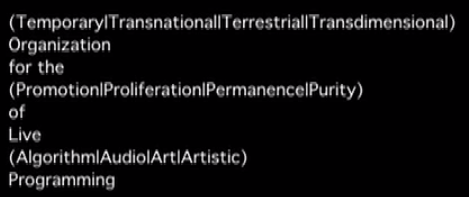
\includegraphics[scale=0.6]{imagens/TOPLAP.png}
  \caption{Definição do siginificado de TOPLAP. \textbf{Fonte}: \citeonline{ramsay_algorithms_2010}.}
  \label{fig:TOPLAP}
\end{figure}

O símbolo ``|'' é uma representação gráfica do operador lógico \emph{OR} (OU), bastante utilizado em algoritmos condicionais. Isto é, \emph{Temporary }| \emph{Trasnational} | \emph{Terrestrial} | \emph{Transdimensional} significa que as letras ímpares ``T'', e ``P'' e ``A'', podem significar um ou outro termo indicado pelo algoritmo.

Este comportamento, de permutar ordem das letras é praticado por Nick Collins (1975-); a permutação de suas letras é utilizada pelo pesquisador para gerar pseudônimos como Click Nilson, ou Sick Lincoln. Isso transparece uma técnica de uso frequente na improvisação de códigos, provavelmente pela facilidade de sua implementação computacional em amb. Por exemplo, o \emph{SuperCollider} oferece um método chamado \emph{scramble}, que embaralha a ordem de um conjunto (de caracteres). Mais especificamente, a permutação de letras transparece uma reorganização gramatica, mas que também reflete em técnicas de reorganização algorítmica da gramática musical.

\subsection{\emph{Show us your screens}}\label{sec:showusyourscreens}

Além das performances inaugurais nos festivais Europeus, o manifesto Lubeck04, \traducao{iniciado em um ônibus de trânsito Ryanair\disponivelem{https://www.ryanair.com/pt/pt/}, em  Hamburgo, para o aeroporto Lübeck\cite[p.~247]{ward_live_2004}}{begun on a Ryanair transit bus from Hamburg to Lubeck airport}, mais conhecido como ``\emph{Show us your screens}'', prescreve algumas regras práticas do \emph{live coding}. 

\begin{citacao}
Exigimos:

• Acesso à mente do intérprete, para todo o instrumento humano.

• Obscurantismo é perigoso. Mostre-nos suas telas.

• Programas são instrumentos que podem modificar eles mesmos.

• O programa será transcendido - Língua Artificial é o caminho.

• O código deve ser visto assim como ouvido, códigos subjacentes visualizados bem como seu resultado visual.

• Codificação ao vivo não é sobre ferramentas. Algoritmos são pensamentos. Motosserras são ferramentas. É por isso que às vezes algoritmos são mais difíceis de perceber do que motosserras.

Reconhecemos contínuos de interação e profundidade, mas preferimos:

• Introspecção dos algoritmos.

• A externalização hábil de algoritmo como exibição expressiva/impressiva de destreza mental.

• Sem \emph{backup} (minidisc, DVD, safety net computer).

Nós reconhecemos que:

• Não é necessário para uma audiência leiga compreender o código para apreciar, tal como não é necessário saber como tocar guitarra para apreciar uma performance de guitarra.

• Codificação ao vivo pode ser acompanhada por uma impressionante exibição de destreza manual e a glorificação da interface de digitação.

• Performance envolve contínuos de interação, cobrindo talvez o âmbito dos controles, no que diz respeito ao parâmetro espaço da obra de arte, ou conteúdo gestual, particularmente direcionado para o detalhe expressivo. Enquanto desvios na tradicional taxa de reflexos táteis da expressividade, na música instrumental, não são aproximadas no código, por que repetir o passado? Sem dúvida, a escrita de código e expressão do pensamento irá desenvolver suas próprias nuances e costumes. 
\footnote{\loccit{ward_live_2004}. Tradução nossa de:\emph{We demand: \begin{inparaenum}[•]
\item Give us access to the performer's mind, to the whole human instrument.
\item Obscurantism is dangerous. Show us your screens.
\item Programs are instruments that can change themselves.
\item The program is to be transcended - Artificial language is the way.
\item Code should be seen as well as heard, underlying algorithms viewed as well as their visual outcome.
\item Live coding is not about tools. Algorithms are thoughts. Chainsaws are tools. That's why algorithms are
sometimes harder to notice than chainsaws.
\end{inparaenum}. We recognise continuums of interaction and profundity, but prefer:  \begin{inparaenum}[•]
\item Insight into algorithms
\item The skillful extemporisation of algorithm as an expressive/impressive display of mental dexterity
\item No backup (minidisc, DVD, safety net computer)
\end{inparaenum}. We acknowledge that: \begin{inparaenum}[•]
\item It is not necessary for a lay audience to understand the code to appreciate it, much as it is not necessary
to know how to play guitar in order to appreciate watching a guitar performance.
\item Live coding may be accompanied by an impressive display of manual dexterity and the glorification of the
typing interface.
\item Performance involves continuums of interaction, covering perhaps the scope of controls with respect to
the parameter space of the artwork, or gestural content, particularly directness of expressive detail. Whilst
the traditional haptic rate timing deviations of expressivity in instrumental music are not approximated in
code, why repeat the past? No doubt the writing of code and expression of thought will develop its own
nuances and customs.
\end{inparaenum}}}
\end{citacao}

Escolhemos dois pontos de interesse ; as frase ``Obscurantismo é perigoso. Mostre-nos suas telas'' e  ``Algoritmos são pensamentos, motosserras são ferramentas'',  foi muito discutida no processo de qualificação desta tese. O primeiro questiona: é realmente necessário a projeção dos códigos para a questão da performance, do ponto de vista musical/cênico?

\subsubsection{Obscurantismo é perigoso, mostre-nos suas telas}\label{sec:obscurantismo}

O manifesto acima surgiu, entre outros motivos, como uma resposta ao artigo ``\emph{Using Contemporary Technology in Live Performance; the Dilemma of the Performer}'' \cite{schloss_dilemma_2003}. A crítica principal de \citeauthoronline{ward_live_2004} refere-se ao sétimo dos questionamentos sugeridos para uma performance de improvisação ao vivo com computadores. Isto é, em um contexto de embate acadêmico, o desafio colocado por \citeonline[p.~241]{schloss_dilemma_2003} foi um estímulo considerável para  emancipação da improvisação de códigos. É curioso notar que o problema e a intenção de Schloss eram opostas ao que foi proposto por \citeauthoronline{ward_live_2004}:


\begin{citacao}
\traducao{Para reiterar, agora que nós temos computadores rápidos o suficiente para execução ao vivo, nós temos novas possibilidades, e um novo problema. Do começo da evidência arqueológica da música até agora, música era tocada acusticamente, e sempre foi fisicamente evidente como o som era produzido; alí existia uma relação de proximiidade entre gesto e resultado. Agora nós não temos mais que seguir as leis da física (ultimamente temos, mas não nos termos do que o observador vê), uma vez que nós temos completo poder do computador como intérprete e intermediário entre nosso corpo físico e o som produzido. \textbf{Por esta causa, a ligação entre gesto e resultado foi completamente perdido, se é que existe ligação. Isto significa que nós podemos ir além da relação de causa-e-efeito entre executante e instrumento que faz a mágica.} Mágica é bom; muita mágica é fatal.}{
To reiterate, now that we have fast enough computers toperform live, we have new possibilities, and a new problem.From the beginning of the archeological evidence of musicuntil now, music was played acoustically, and thus it wasalways physically evident how the sound was produced; there was a nearly one-to-one relationship between gesture andresult. Now we don’t have to follow the laws of physicsanymore (ultimately we do, but not in terms of what theobserver observes), because we have the full power of computers as interpreter and intermediary between our physicalbody and the sound production. Because of this, the link between gesture and result can be completely lost, if indeed there is a link at all. This means that we can go so far beyond the usual cause-and-effect relationship between performer and instrument that it seems like magic. Magic is great; too much magic is fatal
} 
\end{citacao}

A crítica de \citeonline[p.~239]{schloss_dilemma_2003}: \traducao{considerar a visão do observador sobre os modos de performance das interações físicas e mapeamentos de gestos em som, para fazer uma performance convincente e efetiva}{Its now necessary, (\ldots) ;to consider the observer’s view of the performer’s modes of physical interactions and mappings from gesture to sound, in order to make the performance convincing and effective.} era especificamente direcionada aos compositores que improvisam música computacional no palco com foco apenas no aspecto sonoro ou tecnológico. Sua questão tange a ausência de gestos referenciais, esforço físico, no caso de performances com dispositivos extendidos, o problema do movimento exagerado, e a expectativa cênica na performance musical:


\begin{citacao}
\traducao{1. Causa-e-efeito é importante, pelo menos para o observador/audiência em uma sala de concerto. 
\ \\
2.Corolário: Mágica na performance é bom. Muita mágica é fatal! (chato).
\ \\
3. Um componente visual é essencial para a audiência, tal como existe um aparato visual de entrada para parâmetros e gestos.
\ \\
4. Sutileza é importante. Grandes gestos são facilmente visíveis de longe, o que é bom, mas eles são movimentos de desenho animado se comparados à execução de um instrumento musical.
\ \\
5. Esforço é importante. Neste sentido, nós estamos em desvantagem de desempenho na performance musical com o computador.
\ \\
6. Improvisação no palco é bom, mas ``mimar'' o aparato no palco não é improvisação, é edição. É provavelmente mais apropriado fazer isso no estúdio antes do concerto, ou se durante o concerto, com o console no meio ou atrás da sala de concerto.
\ \\
7. Pessoas que representam devem representar. Um concerto de música de computador não é uma desculpa/oportunidade para um programador(a) se sentar no palco. Sua presença melhora ou impede o desempenho da representação?
}{1. Cause-and-effect is important, at least for the observer/audience in a live concert venue. 2. Corollary: Magic in a performance is good. Too much magic is fatal! (Boring). 3. A visual component is essential to the audience, such that there is a visual display of input parameters/gestures. The gestural aspect of the sound becomes easier to experience. 4. Subtlety is important. Huge gestures are easily visible from far away, which is nice, but they are cartoon- movements compared to playi
ng a musical instrument. 5. Effort is important. In this regard, we are handicapped in computer music performance. 6. Improvisation on stage is good, but “baby-sitting” the apparatus on stage is not improvisation, it is editing. It is probably more appropriate to do this either in the studio before the concert, or if at the concert, then at the console in the middle or back of the concert hall. 7. People who perform should be performers. A computer music concert is not an excuse/opportunity for a computer programmer to finally be on stage. Does his/her presence enhance the performance or hinder it?} 
\end{citacao}

Duas opiniões divergentes resolvem seus problemas de maneiras divergentes sem considerarem como uma pode auxiliar a outra. No item 3, é apontado uma questão: para a audiência, e não para o improvisador, o componente visual é essencial (substantificação provável da prática). Ward et al. vão no caminho oposto ao de Schloss, e exageram este item, ao projetar códigos. Mas para Schloss, realizar isso é mimar o aparato (e o público), e tornar a apresentação pedante. É curioso notar, que Schloss faz um apontamento importante, no item 5, sobre a ausência de esforço. Não que ela seja premissa para o resultado sonoro. Mas para o público, e Schloss trata exatamente deste ponto na performance musical (item 1). Mas a crítica mais ácida é o item 7, cujo pensamento não difere de uma lógica fordiana: as atividades de artista e de programador devem ser bem definidas, e separadas. Para Schloss, são duas atividades que não se complementam. Para McLean, são interdisciplinares.


\subsection{Algorithms are Thoughts, Chainsaws are Tools}

``Algorithms are Thoughts, Chainsaws are Tools'' é o nome dado ao vídeo de Stephen \citeonline{ramsay_algorithms_2010}, publicado no Vimeo, em  27 de fevereiro de 2010, como um \emph{Coffee-Table Movie}. É uma análise pessoal da performance de \emph{Strange Places} de Andrew Sorensen. O nome do vídeo é derivado de uma das regras práticas apresentadas na \autoref{sec:showusyourscreens}, p. \pageref{sec:showusyourscreens}; mais especificamente, o sexto item.

O algoritmo como pensamento é um espaço conceitual abstrato \ver{cap:metodologia}; pode conter qualquer fundamento teórico pertinente para uma improvisação específica. O dispositivo usado (motoserra, máquina de tecelagem ou o computador) é um meio pelo qual uma estratégia transversal \ver{sec:imagem_mental} toma sua forma sonora. É interessante aqui notar que este vídeo contém uma descrição e comentários que podem elucidar a frase-alvo sob o prisma da partitura musical. Abaixo realizei uma compilação de fragmentos de alguns dos comentários que considerei pertinentes. Ramsey apresenta a seguinte descrição do vídeo:

\begin{citacao}
Um curta sobre \emph{livecoding} apresentado como parte do Grupo de Estudos de Crítica de Códigos, em 2010, por Stephen Ramsay. Apresenta uma leitura ao vivo $[$\emph{live reading}$]$ de uma performance do compositor Andrew Sorensen. Também fala sobre J.D. Salinger, the Rockets, tocando instrumentos, Lisp, do clima em Brisbane e tímpanos \footnote{\loccit{ramsay_algorithms_2010} Tradução de \emph{A short film on livecoding presented as part of the Critical Code Studies Working Group, March 2010, by Stephen Ramsay. Presents a "live reading" of a performance by composer Andrew Sorensen. It also talks about J. D. Salinger, the Rockettes, playing musical instruments, Lisp, the weather in Brisbane, and kettle drums.}.}.
\end{citacao}

Sem entrar em méritos críticos do registro, limitamo-nos a descrever como um VLog, uma variante no formato audiovisual de \emph{weblogs}\footnote{\cfcite{baker_origins_2008}.}. Se caracteriza por ser um vídeo de curta duração, com opiniões pessoais de quem fez, geralmente no quarto da pessoa, com \emph{headsets} (microfone+headphones). A prática de inserir comentários em um é bastante útil para levantar outras opiniões. Realizamos a tradução de alguns comentários. Não são nossas opiniões, mas podem oferecer ao leitor uma abrengência sobre o que pensam um público entusiasta.

Amanda French nega a utilização do termo \emph{partitura} para explicitar diferenças no uso da programação-partitura, em uma performance de improvisação com o computador, para uma performance não-improvisada com partitura.

\begin{citacao}
A noção de partitura não se aplica aqui, é como não fosse possível aplicá-lo ao músico de \emph{jazz} ou tocador de \emph{bluegrass}. (\ldots). Levanta a questão, para mim, se, em uma sessão de \emph{livecoding} *feita*, constite simplismente no ato de digitar em um programa existente, seria tão convincente -- eu acho que isso pode definitivamente ter pontos de interesse. Ou qual seria o análogo do \emph{livecoding} para uma performance não-improvisada de música?\footnote{\loccit{ramsay_algorithms_2010} Tradução parcial de \emph{The notion of "sheet music" doesn't apply here, as it wouldn't apply to a jazz musician or a bluegrass picker. Even the name of his environment, Impromptu, makes that point. Raises the question for me precisely of whether a livecoding session that *did* consist of simply typing in an existing program would be as compelling -- I think it would definitely have its points of interest, actually. Or what would the livecoding analog be to a non-improvisational live performance of music?}}
\end{citacao}

Um segundo comentário de Matt King, coloca a pergunta de Amanda em outra perspectiva:

\begin{citacao}
O que torna o \emph{livecoding} diferente, e pode a performance de música tradicional imitar isso? Para responder esta questão, parece importante notar que as formas nas quais a música improvisada muitas vezes apela para alguma noção de autenticidade ou gênio. Enquanto o \emph{livecoding} ele mesmo à noção de virtuosismo de código, ``autenticidade'' parece fora de lugar aqui. Se música improvisada sugere expressão, o \emph{livecoding} sugere um conjunto de restrições na expressão, descrevendo os parâmetros através dos quais a máquina $[$midi$]$ ganha expressão \footnote{Tradução nossa de \emph{(\ldots) What makes livecoding different, and can a traditional music performance mimic it? To answer this question, it seems important to note the ways in which improvised music often appeals to some notion of authenticity or genius. While livecoding might lend itself to some notion of coding virtuosity, "authenticity" seems out of place here. If improvised music is expression, livecoding suggests a setting of constraints on expression, describing the parameters through which the machine (midi) gets expressed.}}
\end{citacao}

Michel Pasin defende que o ato de improvisação musical requer conhecimentos técnicos prévios, mas não necessariamente correlacionados ao conhecimento do que é uma partitura: \traducao{Em geral, é somente dominando um instrumento que você pode esquecer sobre a técnica e concentrar em 'dizer' coisas com o instrumento.}{In general, it is only by mastering an instrument that you can forget about the technique and concentrate on 'saying' things with the instrument.}. Este caso é bastante específico de performances com linguagens de baixo e alto-nível. Porém seria possível objetar que a prática de construção de linguagens artificiais, no topo de outras linguagens artificiais, possibilita um praticante não-familiarizado com a programação elaborar rotinas computacionais.  Porém aí caímos em um problema: estaria o praticante realizando uma improvisação de códigos? ou melhor, isso importa, se o objetivo é a criação musical? Para delinear estas questões buscamos definir no próximo capítulo o que consideramos por objetivo de um agenciamento sonoro improvisado.

\section{Discussão}

Oferecemos um cenário proto-histórico do ponto de vista, na Itália com o compositor Pietro Grossi, nos EUA com Jim Horton, John Bischoff, Tim Perkis, e na Holanda com Ron Kuivila (residente nos EUA), que deram suporte ao pensamento promovido na Inglaterra e Alemanha. Sugestões para essa proto-história foram colocados no \autoref{app:B}. Na 